\documentclass{article}

\usepackage[margin=1.2cm, top=1cm, bottom=1.8cm]{geometry}
\pagestyle{plain}
\linespread{1.4}

\usepackage{fontspec}
\usepackage{unicode-math}
\usepackage[main=greek, english]{babel}

\setmainfont{CMU Serif}
\setsansfont{CMU Sans Serif}
\setmonofont{CMU Typewriter Text}
\setmathfont{Latin Modern Math}

\usepackage{amsmath, enumitem}
\usepackage{dirtytalk, caption, subcaption, array, graphicx}
\usepackage{titlesec}
\usepackage{soul}
\usepackage[unicode]{hyperref}

\usepackage{pdfpages}

\usepackage{tikz}
\usetikzlibrary{arrows.meta, positioning}

\hypersetup{
    hidelinks,
    bookmarksopen=true,
    bookmarksnumbered=true,
    pdftitle={Συστήματα Αναμονής - 2η Εργαστηριακή Άσκηση},
    pdfauthor={Πέππας Μιχαήλ-Αθανάσιος}
}

\newcolumntype{P}[1]{>{\centering\arraybackslash}p{#1}}
\titleformat*{\subsubsection}{\large\bfseries}

\begin{document}

\begin{center}
    {
    \Large
    {
    \textbf{ΕΘΝΙΚΟ ΜΕΤΣΟΒΙΟ ΠΟΛΥΤΕΧΝΕΙΟ\\
    ΣΧΟΛΗ ΗΛΕΚΤΡΟΛΟΓΩΝ ΜΗΧΑΝΙΚΩΝ\\
    ΚΑΙ ΜΗΧΑΝΙΚΩΝ ΥΠΟΛΟΓΙΣΤΩΝ\\}
    }

    \vspace{1.5cm}
    \rule{18cm}{0.5pt}

    Τομέας Επικοινωνιών, Ηλεκτρονικής και Συστημάτων Πληροφορικής\\
    Εργαστήριο Διαχείρισης και Βέλτιστου Σχεδιασμού Δικτύων Τηλεματικής - NETMODE\\

    \rule{18cm}{0.5pt}

    \textbf{Συστήματα Αναμονής}\\
    \textbf{$\mathbf{2^{η}}$ Εργαστηριακή Άσκηση}\\
    }
\end{center}

\vspace{0.8cm}
\begin{center}
\includegraphics[width=7cm]{EMP Logo.png}
\end{center}

\Large
{
\vspace{0.8cm}
\noindent
\textbf{Στοιχεία Φοιτητή}
\begin{itemize}
    \item Όνομα: Πέππας Μιχαήλ-Αθανάσιος
    \item Αριθμός Μητρώου: 03121026
    \item $3^{\eta}$ Εργαστηριακή Ομάδα (Δευτέρα, 12:45-14:30)
    \item Ημερομηνία Διεξαγωγής Εργαστηρίου: 16.03.2026
    \item Ημερομηνία Παράδοσης Αναφοράς: 18.03.2026
\end{itemize}
}

\newpage

\tableofcontents

\newpage
\section{Θεωρητική μελέτη της ουράς Μ/Μ/1}

\subsection{Ερώτημα α΄}

Απαραίτητη συνθήκη ώστε η ουρά Μ/Μ/1 να είναι εργοδική είναι η ένταση φορτίου
(traffic intensity), $\rho$, να είναι μικρότερη της μονάδας. Δηλαδή, απαιτούμε τη
συνθήκη Erlang:
\begin{equation}
\rho = \frac{\lambda}{\mu} < 1
\end{equation}

Παρακάτω, στο Σχήμα \ref{fig:mm1_transition}, σχεδιάζουμε το διάγραμμα
ρυθμού μεταβάσεων της ουράς Μ/Μ/1. Θεωρούμε ομοιόμορφους ρυθμούς αφίξεων
$\lambda$ και εξυπηρέτησης $\mu$, ανεξαρτήτως του πλήθους των πελατών στο
σύστημα.

\begin{figure}[h!]
\centering
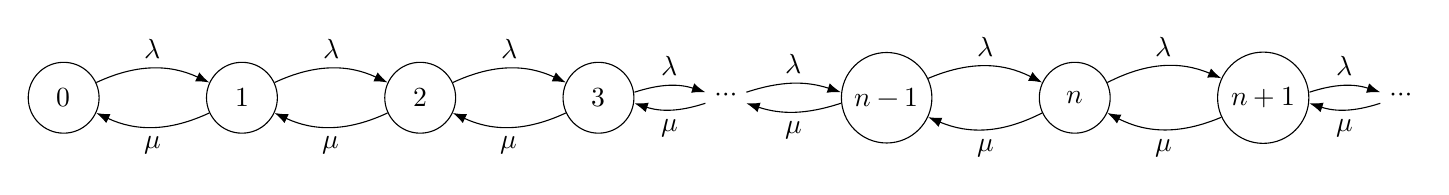
\begin{tikzpicture}[
    >=Latex,
    node distance=1.35cm,
    state/.style={circle, draw, minimum size=9mm},
    every node/.style={font=\normalsize}
]

\node[state] (s0) {$0$};
\node[state, right=of s0] (s1) {$1$};
\node[state, right=of s1] (s2) {$2$};
\node[state, right=of s2] (s3) {$3$};

\node[right=0.9cm of s3] (dots1) {$\cdots$};

\node[state, right=1.2cm of dots1] (sn1) {$n-1$};
\node[state, right=of sn1] (sn) {$n$};
\node[state, right=of sn] (snp1) {$n+1$};

\node[right=0.9cm of snp1] (dots2) {$\cdots$};

% 0 <-> 1
\draw[->] (s0) to[bend left=25] node[above] {$\lambda$} (s1);
\draw[->] (s1) to[bend left=25] node[below] {$\mu$} (s0);

% 1 <-> 2
\draw[->] (s1) to[bend left=25] node[above] {$\lambda$} (s2);
\draw[->] (s2) to[bend left=25] node[below] {$\mu$} (s1);

% 2 <-> 3
\draw[->] (s2) to[bend left=25] node[above] {$\lambda$} (s3);
\draw[->] (s3) to[bend left=25] node[below] {$\mu$} (s2);

% 3 -> ...
\draw[->] ([yshift=2pt]s3.east) to[bend left=18] node[above] {$\lambda$} ([yshift=2pt]dots1.west);
\draw[->] ([yshift=-2pt]dots1.west) to[bend left=18] node[below] {$\mu$} ([yshift=-2pt]s3.east);

% ... -> n-1
\draw[->] ([yshift=2pt]dots1.east) to[bend left=18] node[above] {$\lambda$} ([yshift=2pt]sn1.west);
\draw[->] ([yshift=-2pt]sn1.west) to[bend left=18] node[below] {$\mu$} ([yshift=-2pt]dots1.east);

% n-1 <-> n
\draw[->] (sn1) to[bend left=25] node[above] {$\lambda$} (sn);
\draw[->] (sn) to[bend left=25] node[below] {$\mu$} (sn1);

% n <-> n+1
\draw[->] (sn) to[bend left=25] node[above] {$\lambda$} (snp1);
\draw[->] (snp1) to[bend left=25] node[below] {$\mu$} (sn);

% n+1 -> ...
\draw[->] ([yshift=2pt]snp1.east) to[bend left=18] node[above] {$\lambda$} ([yshift=2pt]dots2.west);
\draw[->] ([yshift=-2pt]dots2.west) to[bend left=18] node[below] {$\mu$} ([yshift=-2pt]snp1.east);

\end{tikzpicture}
\caption{Διάγραμμα μεταβάσεων της ουράς M/M/1.}
\label{fig:mm1_transition}
\end{figure}

Σύμφωνα με το παραπάνω διάγραμμα, γράφουμε τις εξισώσεις ισορροπίας του
συστήματος Μ/Μ/1. Από τις τοπικές εξισώσεις ισορροπίας προκύπτει:
\begin{equation}
\lambda P_0 = \mu P_1 \Rightarrow P_1 = \frac{\lambda}{\mu} P_0 = \rho P_0
\end{equation}
και, γενικότερα:
\begin{equation}
\lambda P_{k-1} = \mu P_k, \quad k \geq 1
\end{equation}
οπότε:
\begin{equation}
P_k = \left(\frac{\lambda}{\mu}\right)^k P_0 = \rho^k P_0, \quad \forall k \geq 1
\end{equation}

Ισοδύναμα, οι σφαιρικές εξισώσεις ισορροπίας γράφονται:
\begin{equation}
(\lambda + \mu)P_k = \lambda P_{k-1} + \mu P_{k+1}, \quad \forall k \geq 1
\end{equation}

Επιπλέον, από την κανονικοποίηση των εργοδικών πιθανοτήτων έχουμε:
\begin{equation}
\sum_{k=0}^{+\infty} P_k = 1
\end{equation}
άρα:
\begin{equation}
P_0 \sum_{k=0}^{+\infty} \rho^k = 1
\end{equation}

Εφόσον $\rho \in (0,1)$, η άπειρη γεωμετρική σειρά συγκλίνει, και συνεπώς:
\begin{equation}
P_0 \cdot \frac{1}{1-\rho} = 1 \Rightarrow P_0 = 1-\rho
\end{equation}

Άρα, οι εργοδικές πιθανότητες των καταστάσεων της ουράς Μ/Μ/1 είναι:
\begin{equation}
P_0 = 1-\rho
\end{equation}
\begin{equation}
P_k = (1-\rho)\rho^k, \quad \forall k \geq 1
\end{equation}

Παρατηρούμε, επίσης, ότι η πιθανότητα το σύστημα να μην είναι άδειο είναι:
\begin{equation}
P\{n(t) > 0\} = 1 - P_0 = \rho
\end{equation}

\subsection{Ερώτημα β΄}

Όπως είναι γνωστό από τη θεωρία, για τις ουρές Μ/Μ/1 ισχύει η σχέση:
\begin{equation}
E[n(t)] = \sum_{k=1}^{+\infty} kP_k = \frac{\rho}{1-\rho}, \qquad \rho = \frac{\lambda}{\mu}
\end{equation}

Έστω ότι η ουρά βρίσκεται σε κατάσταση ισορροπίας. Εφόσον η ουρά Μ/Μ/1 έχει
άπειρη χωρητικότητα, δεν υπάρχουν απώλειες πελατών, και συνεπώς η
ρυθμαπόδοση του συστήματος είναι:
\begin{equation}
\gamma = \lambda
\end{equation}

Άρα, από τον τύπο του Little, ο μέσος χρόνος καθυστέρησης ενός πελάτη στο
σύστημα είναι:
\begin{equation}
E(T) = \frac{E[n(t)]}{\gamma}
      = \frac{E[n(t)]}{\lambda}
      = \frac{1}{\mu - \lambda}
      = \frac{1/\mu}{1-\rho}
\end{equation}

Από τη θεωρία των συστημάτων αναμονής ισχύει:
\begin{equation}
T = W + s
\end{equation}
όπου $W$ είναι ο χρόνος αναμονής στην ουρά και $s$ ο χρόνος εξυπηρέτησης. Επειδή
ο χρόνος εξυπηρέτησης ακολουθεί εκθετική κατανομή με παράμετρο $\mu$, έχουμε:
\begin{equation}
E(s) = \frac{1}{\mu}
\end{equation}

Επομένως, για τον μέσο χρόνο αναμονής ενός πελάτη στην ουρά προκύπτει:
\begin{equation}
E(W) = E(T) - E(s)
     = \frac{1}{\mu - \lambda} - \frac{1}{\mu}
     = \frac{\lambda}{\mu(\mu - \lambda)}
     = \frac{\rho}{\mu(1-\rho)}
\end{equation}

Συνεπώς, ο μέσος χρόνος καθυστέρησης του πελάτη στο σύστημα είναι
$\displaystyle E(T)=\frac{1}{\mu-\lambda}$, ενώ ο μέσος χρόνος αναμονής του στην
ουρά είναι $\displaystyle E(W)=\frac{\rho}{\mu(1-\rho)}$.

\subsection{Ερώτημα γ΄}

Η πιθανότητα να υπάρχουν τουλάχιστον τρεις πελάτες στο σύστημα μία δεδομένη
χρονική στιγμή είναι:
\begin{equation}
P\{n(t) \geq 3\} = \sum_{k=3}^{+\infty} P_k
\end{equation}

Με βάση την έκφραση των εργοδικών πιθανοτήτων, έχουμε:
\begin{equation}
P\{n(t) \geq 3\} = \sum_{k=3}^{+\infty} (1-\rho)\rho^k
\end{equation}

Η πιθανότητα να υπάρχουν τουλάχιστον τρεις πελάτες στο σύστημα είναι το
συμπλήρωμα της πιθανότητας να υπάρχουν το πολύ δύο πελάτες. Επομένως:
\begin{equation}
P\{n(t) \geq 3\} = 1 - \left(P_0 + P_1 + P_2\right)
\end{equation}

Αντικαθιστώντας τις εργοδικές πιθανότητες της ουράς Μ/Μ/1, προκύπτει:
\begin{equation}
P\{n(t) \geq 3\}
= 1 - \left[(1-\rho) + (1-\rho)\rho + (1-\rho)\rho^2\right]
\end{equation}

Άρα:
\begin{equation}
P\{n(t) \geq 3\}
= 1 - (1-\rho)(1+\rho+\rho^2)
= 1 - (1-\rho^3)
= \rho^3
\end{equation}

\subsection{Ερώτημα δ΄}

Η ουρά Μ/Μ/1 έχει άπειρη χωρητικότητα, επομένως κάθε μη αρνητικός ακέραιος
αριθμός πελατών αποτελεί επιτρεπτή κατάσταση του συστήματος. Ειδικότερα, η
κατάσταση με $107$ πελάτες είναι θεωρητικά εφικτή.

Πράγματι, από την έκφραση των εργοδικών πιθανοτήτων προκύπτει:
\begin{equation}
P_{107} = (1-\rho)\rho^{107}
\end{equation}

Για κάθε εργοδικό σύστημα Μ/Μ/1, δηλαδή για κάθε $\rho \in (0,1)$, ισχύει:
\begin{equation}
P_{107} > 0
\end{equation}

Συνεπώς, υπάρχει μη μηδενική πιθανότητα να υπάρξει χρονική στιγμή κατά την
οποία το σύστημα θα βρεθεί με $107$ πελάτες. Βεβαίως, η πιθανότητα αυτή είναι
εξαιρετικά μικρή για συνήθεις τιμές του $\rho$, αλλά αυξάνεται όσο η ένταση
φορτίου $\rho = \lambda/\mu$ πλησιάζει τη μονάδα, δηλαδή όσο ο ρυθμός αφίξεων
πλησιάζει τον ρυθμό εξυπηρέτησης και το σύστημα λειτουργεί πιο κοντά στα όρια
κορεσμού του.

\newpage
\section{Ανάλυση της ουράς Μ/Μ/1 με Octave}

\subsection{Ερώτημα α΄}

Για την ουρά Μ/Μ/1 του παρόντος ερωτήματος, οι αφίξεις ακολουθούν κατανομή
Poisson με μέσο ρυθμό
\[
\lambda = 10 \text{ πελάτες/min}
\]
ενώ ο ρυθμός εξυπηρέτησης \(\mu\) μπορεί να λάβει συνεχείς τιμές στο διάστημα
\([0,20]\) πελάτες/min.

Η απαραίτητη συνθήκη εργοδικότητας της ουράς Μ/Μ/1 είναι:
\begin{equation}
\rho = \frac{\lambda}{\mu} < 1
\end{equation}

Άρα:
\begin{equation}
\frac{10}{\mu} < 1 \Rightarrow \mu > 10
\end{equation}

Λόγω του περιορισμού της εκφώνησης ότι \(\mu \leq 20\) πελάτες/min, οι αποδεκτές
τιμές του ρυθμού εξυπηρέτησης είναι τελικά:
\begin{equation}
10 < \mu \leq 20
\end{equation}

\subsection{Ερώτημα β΄}

Τα ζητούμενα διαγράμματα δημιουργήθηκαν στο Octave με χρήση της εντολής
\texttt{qsmm1()} του πακέτου \texttt{queueing}, για τις επιτρεπτές τιμές του
ρυθμού εξυπηρέτησης \(\mu\).

\begin{figure}[h!]
\centering
\begin{subfigure}[b]{0.48\textwidth}
    \centering
    
\includegraphics[width=\textwidth]{part2_fig1.png}
    \caption{Βαθμός χρησιμοποίησης ως προς το ρυθμό εξυπηρέτησης.}
    \label{fig:mm1_utilization}
\end{subfigure}
\hfill
\begin{subfigure}[b]{0.48\textwidth}
    \centering
    
\includegraphics[width=\textwidth]{part2_fig2.png}
    \caption{Μέσος χρόνος καθυστέρησης ως προς το ρυθμό εξυπηρέτησης.}
    \label{fig:mm1_response}
\end{subfigure}
\caption{Πρώτο ζεύγος διαγραμμάτων για την ουρά Μ/Μ/1.}
\label{fig:mm1_pair1}
\end{figure}

\begin{figure}[h!]
\centering
\begin{subfigure}[b]{0.48\textwidth}
    \centering
    
\includegraphics[width=\textwidth]{part2_fig3.png}
    \caption{Μέσος αριθμός πελατών στο σύστημα ως προς το ρυθμό εξυπηρέτησης.}
    \label{fig:mm1_customers}
\end{subfigure}
\hfill
\begin{subfigure}[b]{0.48\textwidth}
    \centering
    
\includegraphics[width=\textwidth]{part2_fig4.png}
    \caption{Ρυθμαπόδοση πελατών ως προς το ρυθμό εξυπηρέτησης.}
    \label{fig:mm1_throughput}
\end{subfigure}
\caption{Δεύτερο ζεύγος διαγραμμάτων για την ουρά Μ/Μ/1.}
\label{fig:mm1_pair2}
\end{figure}

Από τα παραπάνω διαγράμματα παρατηρούμε ότι ο βαθμός χρησιμοποίησης του
συστήματος μειώνεται μονοτονικά όσο αυξάνεται ο ρυθμός εξυπηρέτησης \(\mu\),
κάτι που είναι θεωρητικά αναμενόμενο, αφού:
\begin{equation}
U = \rho = \frac{\lambda}{\mu}
\end{equation}

Παρατηρούμε, επίσης, ότι τόσο ο μέσος χρόνος καθυστέρησης \(E(T)\), όσο και ο
μέσος αριθμός πελατών \(E[n(t)]\) στο σύστημα μειώνονται πολύ έντονα για τιμές
του \(\mu\) κοντά στο \(10\), και στη συνέχεια η μείωσή τους γίνεται ολοένα και
ηπιότερη καθώς το \(\mu\) αυξάνεται. Η συμπεριφορά αυτή συμφωνεί πλήρως με τη
θεωρία της ουράς Μ/Μ/1, αφού:
\begin{equation}
E(T) = \frac{1}{\mu - \lambda}
\end{equation}
και
\begin{equation}
E[n(t)] = \frac{\rho}{1-\rho} = \frac{\lambda}{\mu-\lambda}
\end{equation}

Συνεπώς, όταν ο ρυθμός εξυπηρέτησης πλησιάζει τον ρυθμό αφίξεων, το σύστημα
λειτουργεί οριακά κοντά στον κορεσμό και οι αντίστοιχες μετρικές αυξάνονται
σημαντικά. Αντίθετα, όσο αυξάνεται το \(\mu\), το σύστημα γίνεται σαφώς πιο
άνετο λειτουργικά.

\subsection{Ερώτημα γ΄}

Με βάση το Διάγραμμα \ref{fig:mm1_response}, παρατηρούμε ότι ο μέσος χρόνος
καθυστέρησης \(E(T)\) μειώνεται καθώς αυξάνεται ο ρυθμός εξυπηρέτησης
\(\mu\). Επομένως, αν λαμβάναμε υπόψη αποκλειστικά και μόνο το κριτήριο της
ελαχιστοποίησης της καθυστέρησης, θα επιλέγαμε τον μέγιστο δυνατό ρυθμό
εξυπηρέτησης, δηλαδή:
\begin{equation}
\mu = 20 \text{ πελάτες/min}
\end{equation}

Παρατηρούμε, όμως, επίσης, ότι όσο το \(\mu\) μεγαλώνει, τόσο ο ρυθμός με τον
οποίο μειώνεται ο μέσος χρόνος καθυστέρησης μειώνεται. Δηλαδή, τα οφέλη από
την περαιτέρω αύξηση του \(\mu\) παρουσιάζουν φθίνουσα απόδοση, ιδίως μετά
από μια περιοχή τιμών όπου η καμπύλη αρχίζει να γίνεται ολοένα και πιο επίπεδη.

Από την πλευρά της σχεδίασης του συστήματος ως μηχανικοί, η αύξηση του ρυθμού εξυπηρέτησης
συνεπάγεται συνήθως και αυξημένο κόστος, είτε σε υποδομή είτε σε πόρους είτε
σε λειτουργικές απαιτήσεις. Επομένως, ως μηχανικοί δεν αναζητούμε απλώς τη
μέγιστη δυνατή τιμή του \(\mu\), αλλά μία ισορροπία ανάμεσα στην ποιότητα
εξυπηρέτησης και στο κόστος υλοποίησης.

Συνεπώς, παρότι η μαθηματικά βέλτιστη επιλογή ως προς το \(E(T)\) είναι το
\(\mu = 20\), πρακτικά μία λογική και συμφέρουσα επιλογή φαίνεται να είναι μία
ενδιάμεση τιμή, περίπου στην περιοχή:
\begin{equation}
12 \leq \mu \leq 14 \text{ πελάτες/min}
\end{equation}
όπου επιτυγχάνεται σημαντική μείωση της καθυστέρησης χωρίς να απαιτείται το
μέγιστο δυνατό κόστος εξυπηρέτησης.

\subsection{Ερώτημα δ΄}

Από το Διάγραμμα \ref{fig:mm1_throughput} παρατηρούμε ότι η ρυθμαπόδοση
του συστήματος παραμένει σταθερή και ίση με:
\begin{equation}
\gamma = 10 \text{ πελάτες/min}
\end{equation}

Αυτό είναι θεωρητικά αναμενόμενο, εφόσον πρόκειται για εργοδική ουρά Μ/Μ/1
απείρου χωρητικότητας. Σε ένα τέτοιο σύστημα δεν υπάρχει πιθανότητα
απόρριψης πελατών, άρα:
\begin{equation}
P_{\text{block}} = 0
\end{equation}

Επομένως, η ρυθμαπόδοση ισούται με το ρυθμό αφίξεων:
\begin{equation}
\gamma = \lambda (1 - P_{\text{block}}) = \lambda = 10 \text{ πελάτες/min}
\end{equation}

Άρα, στην ουρά Μ/Μ/1, όσο το σύστημα παραμένει εργοδικό, η ρυθμαπόδοση δεν
εξαρτάται από το \(\mu\), αλλά παραμένει ίση με το μέσο ρυθμό άφιξης των
πελατών.

\newpage
\section{Διαδικασία γεννήσεων θανάτων: εφαρμογή σε σύστημα Μ/Μ/1/Κ}

\subsection{Ερώτημα α΄}

Θεωρούμε σύστημα αναμονής Μ/Μ/1/3, δηλαδή μαρκοβιανή ουρά με έναν
εξυπηρετητή και μέγιστη χωρητικότητα 3 πελάτες. Σύμφωνα με την εκφώνηση, οι
αφίξεις ακολουθούν κατανομή Poisson με μέσο ρυθμό
\begin{equation}
\lambda_i=\frac{\lambda}{i+2}, \qquad \lambda=5 \text{ πελάτες/sec}
\end{equation}
ενώ ο χρόνος εξυπηρέτησης είναι εκθετικός με σταθερό μέσο ρυθμό
\begin{equation}
\mu_i=\mu=10 \text{ πελάτες/sec}
\end{equation}
ανεξάρτητα από τον αριθμό πελατών στο σύστημα.

Άρα, οι ρυθμοί αφίξεων ανά κατάσταση είναι:
\begin{equation}
\lambda_0=\frac{\lambda}{2}=\frac{5}{2}, \qquad
\lambda_1=\frac{\lambda}{3}=\frac{5}{3}, \qquad
\lambda_2=\frac{\lambda}{4}=\frac{5}{4}
\end{equation}
ενώ οι ρυθμοί εξυπηρέτησης είναι:
\begin{equation}
\mu_1=\mu_2=\mu_3=\mu=10
\end{equation}

Παρακάτω παρουσιάζεται το διάγραμμα ρυθμού μεταβάσεων του συστήματος:

\begin{figure}[h!]
\centering
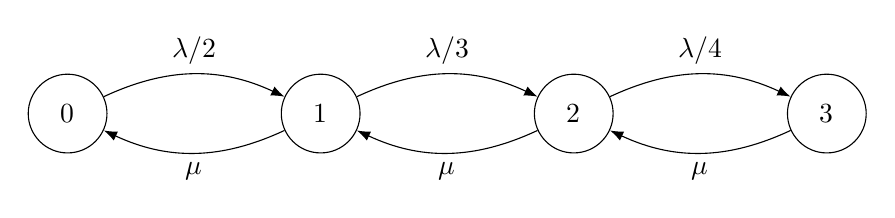
\begin{tikzpicture}[
    >=Latex,
    node distance=2.2cm,
    state/.style={circle, draw, minimum size=10mm},
    every node/.style={font=\normalsize}
]

\node[state] (s0) {$0$};
\node[state, right=of s0] (s1) {$1$};
\node[state, right=of s1] (s2) {$2$};
\node[state, right=of s2] (s3) {$3$};

\draw[->] (s0) to[bend left=25] node[above] {$\lambda/2$} (s1);
\draw[->] (s1) to[bend left=25] node[below] {$\mu$} (s0);

\draw[->] (s1) to[bend left=25] node[above] {$\lambda/3$} (s2);
\draw[->] (s2) to[bend left=25] node[below] {$\mu$} (s1);

\draw[->] (s2) to[bend left=25] node[above] {$\lambda/4$} (s3);
\draw[->] (s3) to[bend left=25] node[below] {$\mu$} (s2);

\end{tikzpicture}
\caption{Διάγραμμα μεταβάσεων της ουράς M/M/1/3.}
\label{fig:mm13_transition}
\end{figure}

Από το παραπάνω διάγραμμα μεταβάσεων προκύπτουν οι λεπτομερείς εξισώσεις
ισορροπίας:
\begin{equation}
\lambda_0 P_0 = \mu_1 P_1
\end{equation}
\begin{equation}
\lambda_1 P_1 = \mu_2 P_2
\end{equation}
\begin{equation}
\lambda_2 P_2 = \mu_3 P_3
\end{equation}
και η εξίσωση κανονικοποίησης:
\begin{equation}
P_0 + P_1 + P_2 + P_3 = 1
\end{equation}

Αντικαθιστώντας τις τιμές των ρυθμών, έχουμε:
\begin{equation}
\frac{\lambda}{2}P_0 = \mu P_1
\Rightarrow
P_1 = \frac{\lambda}{2\mu}P_0
\end{equation}
\begin{equation}
\frac{\lambda}{3}P_1 = \mu P_2
\Rightarrow
P_2 = \frac{\lambda}{3\mu}P_1
= \frac{\lambda^2}{6\mu^2}P_0
\end{equation}
\begin{equation}
\frac{\lambda}{4}P_2 = \mu P_3
\Rightarrow
P_3 = \frac{\lambda}{4\mu}P_2
= \frac{\lambda^3}{24\mu^3}P_0
\end{equation}

Άρα, από την κανονικοποίηση προκύπτει:
\begin{equation}
P_0
\left(
1+\frac{\lambda}{2\mu}+\frac{\lambda^2}{6\mu^2}+\frac{\lambda^3}{24\mu^3}
\right)=1
\end{equation}

Για \(\lambda=5\) και \(\mu=10\) έχουμε:
\begin{equation}
P_0
\left(
1+\frac{5}{20}+\frac{25}{600}+\frac{125}{24000}
\right)=1
\end{equation}
δηλαδή:
\begin{equation}
P_0
\left(
1+\frac{1}{4}+\frac{1}{24}+\frac{1}{192}
\right)=1
\end{equation}

Επομένως:
\begin{equation}
P_0 = \frac{1}{1+\frac{1}{4}+\frac{1}{24}+\frac{1}{192}}
= \frac{192}{249}
= \frac{64}{83}
\approx 0.771084
\end{equation}

Στη συνέχεια, αλυσιδωτά βρίσκουμε:
\begin{equation}
P_1 = \frac{1}{4}P_0 = \frac{16}{83} \approx 0.192771
\end{equation}
\begin{equation}
P_2 = \frac{1}{24}P_0 = \frac{8}{249} \approx 0.032129
\end{equation}
\begin{equation}
P_3 = \frac{1}{192}P_0 = \frac{1}{249} \approx 0.004016
\end{equation}

Άρα, οι εργοδικές πιθανότητες των καταστάσεων του συστήματος είναι:
\begin{equation}
P_0 \approx 0.771084,\qquad
P_1 \approx 0.192771,\qquad
P_2 \approx 0.032129,\qquad
P_3 \approx 0.004016
\end{equation}

Ως γνωστόν από τη θεωρία, η πιθανότητα απόρριψης πελάτη από το σύστημα είναι
η πιθανότητα της τελευταίας κατάστασης, αφού τότε το σύστημα βρίσκεται στη
μέγιστη χωρητικότητά του. Επομένως:
\begin{equation}
P_{\text{blocking}} = P_3 = \frac{1}{249} \approx 0.004016
\end{equation}

\subsection{Ερώτημα β΄}

\subsubsection{Υποερώτημα (i)}

Με τη βοήθεια της εντολής \texttt{ctmcbd} του πακέτου \texttt{queueing} του
Octave, υπολογίζουμε τη μήτρα ρυθμού μεταβάσεων του συστήματος. Με βάση τους
ρυθμούς
\[
\lambda_0=\frac{5}{2},\quad \lambda_1=\frac{5}{3},\quad \lambda_2=\frac{5}{4},
\quad \mu_1=\mu_2=\mu_3=10
\]
η μήτρα ρυθμού μεταβάσεων είναι:
\begin{equation}
Q =
\begin{bmatrix}
-\frac{5}{2} & \frac{5}{2} & 0 & 0 \\
10 & -\frac{35}{3} & \frac{5}{3} & 0 \\
0 & 10 & -\frac{45}{4} & \frac{5}{4} \\
0 & 0 & 10 & -10
\end{bmatrix}
\end{equation}

ή ισοδύναμα σε δεκαδική μορφή:
\begin{equation}
Q =
\begin{bmatrix}
-2.5 & 2.5 & 0 & 0 \\
10 & -11.6667 & 1.6667 & 0 \\
0 & 10 & -11.25 & 1.25 \\
0 & 0 & 10 & -10
\end{bmatrix}
\end{equation}

Παρατηρούμε ότι τα εκτός διαγωνίου μη μηδενικά στοιχεία εκφράζουν τους
ρυθμούς μετάβασης μόνο προς γειτονικές καταστάσεις, όπως ακριβώς αναμένεται
για μια διαδικασία γεννήσεων-θανάτων.

\subsubsection{Υποερώτημα (ii)}

Με την εντολή \texttt{ctmc} του πακέτου \texttt{queueing} βρίσκουμε τις εργοδικές
πιθανότητες των καταστάσεων του συστήματος. Τα αποτελέσματα παρουσιάζονται
παρακάτω, στο Διάγραμμα \ref{fig:mm13_stationary}.

\begin{figure}[h!]
\centering

\includegraphics[width=0.68\textwidth]{part3a_fig1.png}
\caption{Διάγραμμα εργοδικών πιθανοτήτων καταστάσεων της ουράς M/M/1/3.}
\label{fig:mm13_stationary}
\end{figure}

Από την έξοδο του Octave προκύπτουν οι πιθανότητες:
\begin{equation}
P_0 = 0.7710843373,\quad
P_1 = 0.1927710843,\quad
P_2 = 0.0321285141,\quad
P_3 = 0.0040160643
\end{equation}

Οι τιμές αυτές ταυτίζονται πρακτικά με εκείνες που υπολογίστηκαν στο
Ερώτημα α΄, γεγονός που επιβεβαιώνει την ορθότητα της χειρόγραφης επίλυσης.

\subsubsection{Υποερώτημα (iii)}

Η πιθανότητα απόρριψης πελάτη από το σύστημα είναι η πιθανότητα να βρίσκεται
το σύστημα στη μέγιστη χωρητικότητά του, δηλαδή στην κατάσταση \(3\). Άρα:
\begin{equation}
P_{\text{blocking}} = P_3 = 0.004016064257
\end{equation}

Παρατηρούμε ότι η πιθανότητα αυτή είναι πολύ μικρή, κάτι που είναι απολύτως
λογικό, αφού ο ρυθμός εξυπηρέτησης \(\mu=10\) είναι αρκετά μεγαλύτερος από
τους αντίστοιχους ρυθμούς αφίξεων \(\lambda_i\).

\subsubsection{Υποερώτημα (iv)}

Ο μέσος αριθμός πελατών στο σύστημα σε κατάσταση ισορροπίας υπολογίζεται από
τη σχέση:
\begin{equation}
E[n(t)] = \sum_{k=1}^{3} kP_k
\end{equation}

Άρα:
\begin{equation}
E[n(t)] = 1\cdot P_1 + 2\cdot P_2 + 3\cdot P_3
\end{equation}

Αντικαθιστώντας τις εργοδικές πιθανότητες, προκύπτει:
\begin{equation}
E[n(t)] =
1\cdot 0.1927710843
+ 2\cdot 0.0321285141
+ 3\cdot 0.0040160643
\approx 0.2690763052
\end{equation}

Συνεπώς, ο μέσος αριθμός πελατών στο σύστημα όταν αυτό βρίσκεται σε
κατάσταση ισορροπίας είναι:
\begin{equation}
E[n(t)] \approx 0.2691
\end{equation}

\subsubsection{Υποερώτημα (v)}

Στο συγκεκριμένο σύστημα, ο ρυθμός εξυπηρέτησης πελατών είναι σταθερός και
ίσος με \(\mu=10\) πελάτες/sec, αρκεί το σύστημα να μην είναι άδειο. Επομένως,
σε κατάσταση ισορροπίας, η μέση ρυθμαπόδοση εξυπηρέτησης είναι:
\begin{equation}
\gamma = \mu(1-P_0)
\end{equation}

Άρα, για χρονικό διάστημα \(\Delta t = 60\) sec, ο μέσος αριθμός πελατών που
θα εξυπηρετηθεί είναι:
\begin{equation}
N = \gamma \Delta t = \mu(1-P_0)\cdot 60
\end{equation}

Αντικαθιστώντας, έχουμε:
\begin{equation}
N = 10 \cdot (1-0.7710843373)\cdot 60
\approx 137.3493976
\end{equation}

Συνεπώς, ο μέσος αριθμός πελατών που θα εξυπηρετηθεί από το σύστημα σε
60 sec, αφού αυτό βρεθεί σε κατάσταση ισορροπίας, είναι:
\begin{equation}
N \approx 137.35
\end{equation}

\subsubsection{Υποερώτημα (vi)}

Για κάθε μία από τις καταστάσεις του συστήματος σχεδιάζουμε τα διαγράμματα
των πιθανοτήτων των καταστάσεων ως συναρτήσεις του χρόνου από την αρχική
κατάσταση, μέχρι οι πιθανότητες να έχουν απόσταση μικρότερη του \(1\%\) από
τις εργοδικές πιθανότητες. Τα αποτελέσματα φαίνονται στο
Σχήμα \ref{fig:mm13_transient}.

\begin{figure}[h!]
\centering

\includegraphics[width=0.92\textwidth]{part3a_fig2.png}
\caption{Πιθανότητες των καταστάσεων \(0\) έως \(3\) ως συναρτήσεις του χρόνου, μέχρι σύγκλιση στην εργοδική κατάσταση.}
\label{fig:mm13_transient}
\end{figure}

Επειδή το σύστημα είναι αρχικά άδειο, έχουμε:
\begin{equation}
P_0(0)=1,\qquad P_1(0)=P_2(0)=P_3(0)=0
\end{equation}

Παρατηρούμε ότι η πιθανότητα της κατάστασης \(0\) μειώνεται με το χρόνο,
ενώ οι πιθανότητες των υπολοίπων καταστάσεων αυξάνονται μέχρι να πλησιάσουν
τις αντίστοιχες εργοδικές τους τιμές. Από την έξοδο του Octave προκύπτει ότι
όλες οι πιθανότητες βρίσκονται σε απόσταση μικρότερη του \(1\%\) από τις
εργοδικές τιμές τους περίπου στο:
\begin{equation}
t \approx 0.37 \text{ sec}
\end{equation}

Άρα, το συγκεκριμένο σύστημα συγκλίνει αρκετά γρήγορα στην κατάσταση
ισορροπίας.

\subsubsection{Υποερώτημα (vii)}

Στο υποερώτημα αυτό επαναλαμβάνουμε τον υπολογισμό του μέσου αριθμού
πελατών που εξυπηρετούνται σε \(60\) sec για τις περιπτώσεις:
\[
(i)\ \lambda=5,\ \mu=1,\qquad
(ii)\ \lambda=5,\ \mu=5,\qquad
(iii)\ \lambda=5,\ \mu=20
\]
και σχολιάζουμε ποιοτικά πώς μεταβάλλονται οι πιθανότητες και η ταχύτητα
σύγκλισης στην εργοδική κατάσταση.

\begin{figure}[h!]
\centering

\includegraphics[width=0.92\textwidth]{part3b_fig1.png}
\caption{Πιθανότητες των καταστάσεων για την περίπτωση \(\mu=1\).}
\label{fig:mm13_mu1}
\end{figure}

\begin{figure}[h!]
\centering

\includegraphics[width=0.92\textwidth]{part3b_fig2.png}
\caption{Πιθανότητες των καταστάσεων για την περίπτωση \(\mu=5\).}
\label{fig:mm13_mu5}
\end{figure}

\begin{figure}[h!]
\centering

\includegraphics[width=0.92\textwidth]{part3b_fig3.png}
\caption{Πιθανότητες των καταστάσεων για την περίπτωση \(\mu=20\).}
\label{fig:mm13_mu20}
\end{figure}

Από την έξοδο του Octave, για \(\mu=1\) προκύπτουν:
\begin{equation}
P_0=0.077670,\quad
P_1=0.194175,\quad
P_2=0.323625,\quad
P_3=0.404531
\end{equation}
ενώ η πιθανότητα απόρριψης είναι:
\begin{equation}
P_{\text{blocking}}=P_3=0.404531
\end{equation}
και ο μέσος αριθμός πελατών που εξυπηρετούνται σε \(60\) sec είναι:
\begin{equation}
N \approx 55.34
\end{equation}
με χρόνο σύγκλισης περίπου:
\begin{equation}
t \approx 4.39 \text{ sec}
\end{equation}

Για \(\mu=5\) προκύπτουν:
\begin{equation}
P_0=0.585366,\quad
P_1=0.292683,\quad
P_2=0.097561,\quad
P_3=0.024390
\end{equation}
με:
\begin{equation}
P_{\text{blocking}}=0.024390,\qquad
N \approx 124.39,\qquad
t \approx 0.98 \text{ sec}
\end{equation}

Τέλος, για \(\mu=20\) προκύπτουν:
\begin{equation}
P_0=0.880229,\quad
P_1=0.110029,\quad
P_2=0.009169,\quad
P_3=0.000573
\end{equation}
με:
\begin{equation}
P_{\text{blocking}}=0.000573,\qquad
N \approx 143.72,\qquad
t \approx 0.14 \text{ sec}
\end{equation}

Παρατηρώντας τα παραπάνω διαγράμματα και τα αριθμητικά αποτελέσματα,
καταλήγουμε στα εξής βασικά συμπεράσματα.

Πρώτον, καθώς αυξάνεται ο ρυθμός εξυπηρέτησης \(\mu\), η πιθανότητα της άδειας
κατάστασης \(P_0\) αυξάνεται, ενώ οι πιθανότητες των υψηλότερων καταστάσεων,
και ιδιαίτερα της κατάστασης μέγιστης χωρητικότητας \(P_3\), μειώνονται
σημαντικά. Αυτό είναι απολύτως λογικό, αφού όσο ταχύτερα εξυπηρετείται ένας
πελάτης, τόσο δυσκολότερα ``γεμίζει'' το σύστημα.

Δεύτερον, η πιθανότητα απόρριψης πελάτη μειώνεται δραστικά καθώς αυξάνεται το
\(\mu\). Πράγματι, από περίπου \(40.45\%\) για \(\mu=1\), πέφτει σε περίπου
\(2.44\%\) για \(\mu=5\), και γίνεται πρακτικά μηδενική για \(\mu=20\).

Τρίτον, η σύγκλιση προς την εργοδική κατάσταση γίνεται πολύ ταχύτερη όσο
αυξάνεται ο ρυθμός εξυπηρέτησης. Συγκεκριμένα, ο χρόνος σύγκλισης μειώνεται
από περίπου \(4.39\) sec σε \(0.98\) sec και τελικά σε \(0.14\) sec. Άρα, το
σύστημα γίνεται όχι μόνο πιο ``άδειο'' στατιστικά, αλλά και ταχύτερο στη
μετάβασή του προς την ισορροπία.

Τέταρτον, ο μέσος αριθμός πελατών που εξυπηρετούνται σε \(60\) sec αυξάνεται
όταν αυξάνεται το \(\mu\), αλλά όχι αναλογικά με αυτό. Ενώ δηλαδή το \(\mu\)
αυξάνεται πολύ έντονα από \(1\) σε \(20\), ο αντίστοιχος μέσος αριθμός
εξυπηρετούμενων πελατών αυξάνεται από περίπου \(55.34\) σε \(143.72\). Αυτό
συμβαίνει επειδή το σύστημα δεν τροφοδοτείται με σταθερό ρυθμό \(\lambda\),
αλλά με ρυθμούς \(\lambda_i=\lambda/(i+2)\), οι οποίοι μειώνονται όσο
αυξάνεται το πλήθος πελατών στο σύστημα. Επομένως, η άφιξη πελατών αποτελεί
τελικά τον περιοριστικό παράγοντα.

Τέλος, στην περίπτωση \(\mu=1\) παρατηρούμε ότι η πιθανότητα της κατάστασης
\(1\) δεν συγκλίνει μονοτονικά, αλλά παρουσιάζει αρχικά αύξηση πάνω από την
εργοδική της τιμή και στη συνέχεια μειώνεται προς αυτήν. Αυτό είναι λογικό,
καθώς το σύστημα ξεκινά άδειο, δέχεται αρχικά αφίξεις και ``περνά'' πρώτα από
τις χαμηλές καταστάσεις, πριν συσσωρευτεί πιθανότητα στις υψηλότερες
καταστάσεις \(2\) και \(3\).

\newpage
\section{Παράρτημα Υλοποιήσεων σε Octave}

\subsection{Octave Code - Part 2}

\includepdf[pages=-]{lab2_part2.pdf}
\subsubsection{Έξοδος Προγράμματος Part2}
\begin{figure}[h!]
\centering

\includegraphics[width=0.92\textwidth]{part2_output.png}
\caption{Έξοδος Προγράμματος Part2}
\end{figure}

\newpage
\subsection{Octave Code - Part 3a (i-vi)}

\includepdf[pages=-]{lab2_part3a.pdf}
\subsubsection{Έξοδος Προγράμματος Part3a (i-vi)}
\begin{figure}[h!]
\centering

\includegraphics[width=0.92\textwidth]{part3a_output.png}
\caption{Έξοδος Προγράμματος Part3a (i-vi)}
\end{figure}

\newpage
\subsection{Octave Code - Part 3b (vii)}

\includepdf[pages=-]{lab2_part3b.pdf}
\subsubsection{Έξοδος Προγράμματος Part3b (vii)}
\begin{figure}[h!]
\centering

\includegraphics[width=0.8\textwidth]{part3b_output.png}
\caption{Έξοδος Προγράμματος Part3b (vii)}
\end{figure}


\end{document}
